\documentclass[a4paper]{article}
\usepackage[scale=0.75]{geometry}
\usepackage{algorithm,algorithmicx,algpseudocode}
\usepackage{lmodern}
\usepackage{caption}
\usepackage{graphicx}
\usepackage{mathptmx}
\usepackage{mathtools}
\usepackage{algorithm,algorithmicx,algpseudocode}
\usepackage{float}
\usepackage{booktabs}
\usepackage{multirow}
%\usepackage{natbib}
\usepackage{cite}
\usepackage[colorlinks=true,urlcolor=blue,citecolor=black]{hyperref}

\DeclarePairedDelimiter\abs{\lvert}{\rvert}%
\DeclarePairedDelimiter\norm{\lVert}{\rVert}%

\newcommand{\specialcell}[2][c]{%
  \begin{tabular}[#1]{@{}c@{}}#2\end{tabular}}

      

\makeatletter
\let\oldabs\abs
\def\abs{\@ifstar{\oldabs}{\oldabs*}}
\let\oldnorm\norm
\def\norm{\@ifstar{\oldnorm}{\oldnorm*}}
\makeatother

\usepackage{xcolor}


\title{}
\author{Simon Carrignon, Xavi Rubio-Campillo \& Jean-Marc Montanier}
\date{2016}


\begin{document}

\section{Introduction}
Historical sciences have now a rich trajectory of applying computer simulation to answer research questions. They provide the needed methodological tools to evaluate complex scenarios where non-linear trajectories unfold over long-term time spans and where the contingency of events is central.

These computer models have been often classified in three types based on their goal: a) hypothesis-testing, b) tactical simulations and c) theory-building. Most models follow the first option, which allows the research to evaluate the plausibility of working hypotheses against empirical evidence. The second option is focused on testing methodological challenges of the different discipline.

This work examines the epistemological and methodological challenges posed by computer model and simulation in History and Archaeology in general and why we think they can be fruitfully uses to study History by comparing it with Evolutionary Biology. 

We focus here in the third type, which explores abstract scenarios with the aim of generating new ideas and knowledge using a stylized model of the studied system. While it is true that any hypothesis needs to be finally tested against evidence, the heuristics utility of these theory-building in other scenarios clearly shows the potential of this approach for any scientific discipline. 

We will exemplified the utility of this kind of model by presenting an Agent-Based Model exploring the co-evolution of trade and culture within the Roman Empire. This model allows us to explore the dynamics of a simple goods exchange economy under different cultural network constraint.% the second focus on the impact of the learning abilities on the evolution of a Producer/Consumer system.



\section{General issues}


\subsection{Evolutionary Biology}
Incompleteness and uncertainty of the historical and archaeological record affect historical interpretation \cite{madella2014} but \emph{formal modelling} and computer simulation are valuable tools to overcome such limitations. 

Evolutionary Biologists have successfully embraced these tools long time ago and we think that their epistemological framework is close enough to what archaeologists and historians do to be used as an example to follow. 

Indeed, the goal of Evolutionary Biologist is to understand the mechanisms at the origin of the living world as we can observe it. To do so and assuming the theory of evolution by natural selection, they characterise the succession of past events that constitute the Story of Life. Starting with Gould \cite{gould1989wonderfullife}, several biologists and philosophers have argued that the nature of this research activity \emph{is} historical \cite{beatty1995evolutionary}: the actual biological world does not depend \emph{only} on biological rules, but on the uniqueness of the succession of events. To encompass the issues raised by such historicity, evolutionary biologists have developed, since the biometricians and later during the modern synthesis, formal models that help them to explain the patterns they observe in the biological world.  From those formal model, they can figure out different possible successions of events and the likelihood of such possible historical paths given wide range of different data. 

If at first those model were only formal model described as mathematical equation (Wright-Fisher genetic drift model, Hardy Weinberg equilibrium\ldots) the apparition of computer and their spread in Science in general offered biologists new ways to describe the biological world and computational power to explore area impossible to study by other traditional analytics mean (the huge amount of data generated by Genetics and the quick development of Bio-infomatics to manage such data is a good example). Thus, the computational approach was quickly and widely embraced by all fields of Biology in at least to way: (1) to simulate and derive complex dynamical formal models and compare them (numerical simulations), (2) to describe systems where the main properties emerge from the interactions between the subparts of the system and are difficult to describe mathematically (computer modelling).  

By the very nature of the object studied (succession of events producing complex patterns), Evolutionary Biology and History are very close. We think that the tools and methods developed in the first context can and should be applied to study historical problems.
In the following section we will focus on the second type of computer simulation and we will show why they can be of particular interest for historian and archaeologist.

%The more visible example of such use of computer model is exemplified by the major and always growing role played by \emph{Bioinformatics} in a lot of areas in Biology during the last three decades.
%This suggest that (i) the problems encountered by evolutionary biologists are close to those archaeologists and historians have to face (ii) the way inferences are made about the history of living beings and the history of human societies fall into a similar epistemological framework and (iii) mathematical and computer models are good candidates to infer, in a statistically plausible and transparent way, missing data and complex hypotheses in both enterprise.

\subsection{Computer Simulations and Modelling}

As we said before, Evolutionary Biologist use computer simulations for at least two things. Numerical simulation, that allows biologist to simulates complex mathematical model and select between them (as done by people doing Bayesian inference in phylogenetic for example) is already well used by historians and archaeologists (cf  \cite{rubiocampillo2016modelselectioninhistoricalresearchusingapproximatebayesiancomputation} for example). But, in complex systems where the interactions of every subcomponents are multiple, such as in human society where the social-cultural environment interacts with biological and economical evolution, or in Evolutionary Biology where the interaction between development, environment and evolution are central, the global dynamics \emph{emerge} from the interactions of the subparts of the systems. These subparts are often heterogeneous in nature and are interacting in complex retroacting loops making such system difficult to predict analytically and to describe with simple mathematical equation. This make computer modelling (using algorithmic description of the model) one of the best suitable tool to explore and study those mechanisms.

We think that those problem apply to history and archaeology and we want  here  to argue in favor of such models. We will give the example of one of them in the following section.

This use of computer simulations and modelling is not restricted to Evolutionary Biology. It is widely spread in all branches of Science and people studying computer simulation \emph{per se}, in the field which is commonly called ``artificial life''\cite{langton89alifeiproceedingsfirstinternationalworkshopsynthesissimulationlivingsystems} have already thought about simulation and computer model. They have proposed different classifications of computer model the one we want to use have often been described as ``conceptual model'' (\cite{barandiaran06alifemodelsasepistemicartefacts}. Such computer model are powerful heuristic tools that combine the exploratory power of thought experiments and the logical strength of mathematics \cite{paolo00simulationmodelsasopaquethoughtexperiments}.  They allow to test quickly a lot of possible ``opaque though experiments'' that would be impossible to execute mentally. As though experiments, they offer to experimenters a freedom impossible to reach with traditional experiments doing measures directly on the object of study (galaxies in physics, human in psychology,\ldots), while as running on computer, they can handle operation lasting very long timespan and involving range of parameters that one could not handle with his own mind.

They are the perfect tool to generate new hypothesis when few have been proposed, as they allow to deeply explore and compare models and theories without relying on particular data. We think that this is particularly relevant in history and archaeology, where the traditional inductive approach is strongly data driven whereas the uncertainty and the quality of the data cannot really support any of the induced hypothesis and often lead to strong equifinality (many hypothesis can explain the same observed pattern). 

Conceptual computer models seen as thought experiments provide us an artificial lab that can guides us through equifinality  problems, helps us to generate new hypothesis and provides formal arguments to support hypothesis that can hardly be supported by insufficient empirical evidences.

However, building computational simulations that can provide valuable knowledge about the target system still remains a difficult task. Computer scientists have to be aware of every assumptions they could implicitly made and domain experts (as historians or biologists) have to formulate their hypotheses in an epistemological framework yet not clearly specified and far from the one they are used. The communication is thus primordial: knowledge here does not lie in the mathematical models neither in the historical data but emerges from the well articulation of both side \cite{winsberg09taletwomethods}.

We will shown  one example of a model that could be used by historians and archaeologists in order to help them to test and generate hypotheses. This model is very general  and doesn't incorporate  knowledge about a particular target system (in contrary to \cite{brughmans2016mercuryanagentbasedmodeloftablewaretradeintheromaneast}). It allows us to explore general idea about economy and cultural transmission and their interactions in a innovative way, that does not depend on one particular dataset or on particular historical point of view. Moreover it can integrate already formalized model from any other discipline and any knowledge from history and archaeology, to cognitive sciences and economy. It thus gives us a way to weight the likelihood of trillion of different scenarios that will help then to generate new hypothesis about historical process where few hypothesis have been made or where knowledge isn't good enough to build formal model.


%Here we provide examples from the EPNet project, where the emphasis is on supporting historians with computational infrastructure for understanding the political and economical implications behind food production and distribution along the Roman Empire. By taking into consideration the design and development of such a computational infrastructure, the EPNet epistemological framework is aiming to address three main problems: (i) structuring and making accessible large collections of data through the Web, (ii) providing a formally defined, unambiguous, framework for analysing the data and exporting them in a way that can be further manipulated by computer simulation algorithms, and complex network analysis, and (iii) making each collection of data integrable with other complementary data sources.

\section{Example of a Computer Model to study co-evolution of trade \& culture}

This section presents an example of a model to study the co-evolution of cultural change and trade. This model was designed to propose a trade-off between the flexibility necessary for the test of multiple models, that could be based on historical and archaeological assumption, hypothesis and observation and/or actual knowledge on cognition, economy, network theory and so on. This implements the opaque thought experiments we described earlier. It gives us the structure necessary for the in-depth exploration of some general hypothesis made on the transmission of culture and the evolution of economy without relying on one particular dataset or historical knowledge ; and allows for the quantitative comparison between the different models and theories.

To create this framework we propose an Agent-Based Model relying on agents producing, exchanging and associating values to a list of goods. We present the key concepts of the framework and two examples of its implementation which allow us to show the flexibility of our framework. Moreover, we compare the results obtained by the two models, thus validating the structure of the framework. Finally, we validate the implementation of a trading model by studying the price structure it produces.


\subsection{Trade \& Cultural Evolution}\label{sec:tc:intro}


Cultural change comprises the collection of processes that promotes or inhibits the spread of information by social interaction within a population~\cite{boyd_origin_2005}. An increasing number of social scientists are using an evolutionary framework to model cultural change~\cite{henrich_evolution_2003}. This approach aims at fostering the development of transdisciplinary efforts designed to understand cultural change.

Within the studies done in the evolutionary framework, a cultural phenomenon (such as music) is viewed as a collection of traits (such as musical genres). Multiple biases (mechanism favouring the use of a cultural trait over an other) can explain the fact that certain of the cultural traits are transmitted more readily than the others. Among the biases studied, some can be explained by the intrinsic properties of a trait (how beneficial it is for the individual using it), while others are explained by the frequency of these traits (how popular a trait is in the culture). 

Multiple models can be proposed to represent cultural changes, one of them being the neutral model~\cite{neiman_stylistic_1995}. Within this type of model it is assumed that a trait does not bias the fitness of the individual that acquires it. It therefore means that no bias modifies the rate of transmission of the cultural traits, and that their success will depend only on their frequency in the population. Within analysis of real data, a neutral model produces a distinctive type of frequency distribution of cultural traits termed \emph{power law}.
 
The \emph{power law} can be replicated within a virtual setup thanks to a simple random copying transmission mechanism~\cite{bentley_random_2004}: an individual will copy the traits of a randomly chosen individual with a given probability. This copy can potentially introduce some errors in the acquired trait, which account for innovation processes. The individual will in turn continue to spread these cultural traits which will be further adopted by other individuals. This basic model can be enriched by several additional processes both in the innovation~\cite{schillinger_copying_2014,sole_evolutionary_2013,ziman_technological_2003} and the transmission~\cite{heyes_social_1994,henrich_evolution_2003}. Unbiased transmission works as a baseline for identifying frequency-dependent biases: if evidence has higher tendency to copy the most common trait it is known as conformism, while the opposite is defined as anti-conformism.

The archaeological record allows the researchers to identify frequency-dependence biases on cultural transmission over long-term trajectories~\cite{lipo_neutralitystyle_2001,shennan_ceramic_2001,steele_ceramic_2010}. However, the fact that material culture recovered from archaeological contexts is noisy and fragmented presents some challenges on the validity of the method~\cite{kandler_nonequilibrium_2013,porcic_exploring_2014,crema_approximate_2014}

This work explores the impact of a crucial element on the transmission of material culture: trade. Networks of good exchanges are being increasingly recognised as key elements that structured ancient societies~\cite{temin_market_2001,remesal_epnet_2014,brughmans_connecting_2010}. The scenarios where this process emerges suggest a complex bias in the selection of cultural traits, which at the same time are also identified as economic goods~\cite{bentley_specialisation_2005,macmillan_agent-based_2008}. Transmission is not neutral anymore, as different prices for each good will introduce a dynamic content bias. This affects the frequency of the good within the population, which in turn modifies its price following a co-evolutionary dynamic.

These dynamics are studied using an Agent-Based Model (ABM), a type of simulation particularly useful for studying non-linear dynamics in heterogeneous environments within an evolutionary perspective~\cite{lake_trends_2014}. More precisely we propose a framework that can be implemented in multiple ways depending on the model tested. Next subsection defines the framework, which is based on the basic processes found in evolutionary models of cultural change. Next, we define the implementations used to explore the dynamics of the created framework. In the following subsection we analyse the results obtained with these two implementations. Finally, the concluding remarks discuss further possibilities of the presented framework.

\subsection{Framework Description}

To explore the co-evolution between trade and cultural change we have developed a framework where the different agents produce and trade goods to which they assign variable values. The model is composed of a population $Pop$ of $m$ agents, each defined by 2 vectors of size $n$. The first corresponds to the quantity of each good owned by the agent $i$: 
$$\forall i \in Pop, \quad Q^i = (q^i_1,\cdots,q^i_n) $$
where $Q^i$ is the total list of possessions of agent $i$, and $q^i_j$ is the number of goods of type $j$ that agent $i$ possesses.

The second vector reflects the estimation of the value of a good made by an agent $i$:
$$\forall i \in Pop, \quad V^i = (v^i_1,\cdots,v^i_n) $$
where $V^i$ is the total list of estimated values of agent $i$, and $v^i_j$ is the value that agent $i$ associates to one unit of a good of type $j$.

On top of these elements five processes are used: \emph{production}, \emph{consumption}, \emph{cultural transmission}, \emph{innovation} and \emph{trade}. The \emph{production} process describes the creation of goods by the agent. Once a good is produced by an agent $i$ it is added to its quantity vector ($Q^i$). The consumption strategy of these goods is defined in the \emph{consumption} process which decreases the number of goods in the vector ($Q^i$). In this model, all goods are completely consumed at each iteration for all the models tested. The \emph{trade} process models the exchange of goods between the agents which results in a modification of the quantity vectors ($Q^i$). The amount of goods exchanged is computed by the agents involved in the trade, within the \emph{trade} process, based on their value vectors ($V^i$). Within the \emph{cultural transmission} process an agent $i$ can copy the entire value vector ($V^j$) of an agent $j$, where $j \neq i$. Finally, the \textit{innovation} process also modifies the value vector $V^i$ of an agent, but it differs from the \emph{cultural transmission} process in that the modification is done without reference to the other agents.

The scheduling of the five processes is described in algorithm~\ref{algo:complete} along with the vectors modified by each of these processes. On lines 3 and 4 all agents of the population are initialised with empty quantity vectors and random values. The code used to update the status of each agent at each iteration is presented between the lines 8 and 22. One can note that each of the five processes is executed synchronously by all agents. Moreover, the \emph{trade} process is called at each iteration while the \emph{cultural transmission} and \emph{innovation} processes are executed only every $CulturalStep$. The idea behind this is to perform the \emph{cultural transmission} based on a score that reflects the performance of the agent and not only one lucky or unlucky trading round. The timestep number used in all the figures presenting the results of this model refers to the number of times the \emph{cultural transmission} and \emph{innovation} processes are called.

\begin{algorithm}
\caption{Model}
\label{algo:complete}
	\begin{algorithmic}[1]
	\State INITIALIZATION: 
		\For{$i \in \#Pop$} \Comment{Initialize the agent with no goods and a random value vector}
				\State $Q^i = (0, \cdots, 0)$
				\State $V^i = (v^i_0, \cdots, v^i_n)$ \Comment{The values of $v^i_j$ are selected randomly}
		\EndFor

	\State SIMULATION:
		\Loop{$~step \in TimeSteps$}
			\For{$i \in Pop$}
				\State $Production(Q^i)$
			\EndFor
			\For{$i \in Pop$}
				\For{$j \in Pop$}
					\State $TradeProcess(V^i,Q^i,V^j,Q^j)$
				\EndFor		
			\EndFor
			\For{$i \in Pop$}
				\State $ConsumeGoods(Q^i)$ \Comment{All goods are consumed}
				\If{$ (step \mod CulturalStep) = 0$}	
					\State $CulturalTransmission(V)$
					\State $Innovation(V^i)$
				\EndIf
			\EndFor
		\EndLoop
\end{algorithmic}
\end{algorithm}


In order to validate our model we first reproduce common results from the literature on cultural transmission. We then show that it is possible to transform our model to fit processes that are economically sound, i.e. the model should show the convergence optimal values such as shown in~\cite{gintis_emergence_2006}. To achieve these two goals, we have designed for each one a specific set of implementations of the five core processes (production, consumption, trade, cultural transmission and innovation). 


\subsubsection{Neutral Configuration}\label{sec:tc:culturalTrans}

The first scenario is designed to reproduce unbiased transmission, where each good is a cultural trait without intrinsic positive or negative weight \cite{bentley_random_2004,bentley_specialisation_2005,mesoudi_random_2009}. 
Under this hypothesis, the processes of \emph{production} and \emph{trade} are not relevant, and as a consequence, they do not modify the content of the quantity vectors of the agents.


Unbiased \emph{cultural transmission} is implemented using ``random copy'': each agent has a low probability to pick randomly one agent among all and copy its vector of values. The \emph{innovation} process, termed ``unbounded'', is triggered with a low probability ($\mu$) and draw a new random value to replace an element $v^i_j$.

The neutral hypothesis states that the ``random copy'' transmission and the ``unbounded'' innovation process used under a fixed population size leads to a distribution of frequency of cultural variants termed \emph{power law}. This distribution is characterized by a small number of very frequent traits and a large number of rare traits. The main difference with similar distributions, such as exponential distribution, is that the rare traits are far from being absent of the distribution, i.e. the tail of the distribution is large.

This distribution is formalised as : $$P(v)=C/v^\alpha $$ where $v$ is the number of times a variant has been repeated, $P(v)$ the probability to find that variant, $C$ a constant, $\alpha$ a variable describing the slope of the curve obtained. We will therefore attempt to fit as well as possible the results obtained with this set of implementations to the ``power law'' distribution by modifying the $\alpha$ parameter.

\subsubsection{Trading Biased Configuration}\label{sec:tc:trade}

In the second scenario, we are interested in the exchange of goods between agents in a barter process where each agent can choose its prices of exchange. We want to implement simple processes leading to the convergence of all prices to values acceptable by all agents, i.e. we would like to observe, at the end of an experiment, all the agents using a set of prices which allow them to trade efficiently.

\paragraph{Production} Each agent produces one good. The type of good produced by an agent $i$ is assigned to it at the beginning of the simulation, does not change through the simulation, and is referred to as $produced^i$. At each time step, each agent, produces a number of units (of its production good) equal to the number of goods, which ensures that enough is owned to be traded for other goods. Moreover, when an agent consumes its own production good, it does not impact its inventory.

\paragraph{Cultural transmission}
Social learning is here biased towards the agents which are the best at trading, and is therefore termed ``success bias''. To achieve this bias, the cultural transmission mechanism used takes into account the value vector of the other agents and relies on two new notions: \emph{need} and \emph{score}. 

The \emph{need} is a quantity of good that each agent tries to obtain. This quantity is different for each good but the need for a good is the same for all agents:
$$ N = (n_1, \cdots, n_r) $$ 

The \emph{score} $s^i_j$ of an agent $i$ reflects the ability of this agent to obtain the quantity of good $j$ it needs. It is maximum when the quantity $q^i_j$ that an agent $i$ owns of the good $j$ is equal to the need $n_j$ for the good $j$ and lowers proportionally to the distance between the need vector and the quantity vector. It is calculated in such a way that each good has the same weight in the final score, i.e. managing to get only the right amount of a good with a high ``need'' value will not give a better score to the agent and is formal description is given in the Annex

The complete score of an agent $i$ is termed $s^i$ and corresponds to the sum of the $s^i_j$. An agent will choose from whom the price vector should be copied among the agents that produce the same good and have the highest score. In practice, the worst (in terms of score) 20 percent of the agents producing the same good will copy the prices of the best twenty percent producing the same good. The algorithmic description of this selection process is given in the Annex with the algorithm~\ref{algo:selectionCulture}.


\paragraph{Trading} 
During the trading phase the value associated to a good by an agent corresponds to the subjective price of the good for this agent. Briefly summarised, for each good that it does not produce, an agent will trade with the first partner that offers an acceptable trade, i.e. an agent that proposes a satisfiable ratio between the other good and the good produced by the agent. 

If a trade is possible, the two agents will exchange the agreed quantities. If the trade is not possible, the agent will continue to look at random partners for this good until either a partner is found or $TradeThreshold$ agents have been tried. At this point the agent will try to trade with agents producing another good. The process goes on until all goods have been tried. This trading process is described in the algorithm~\ref{algo:trade} in the Annex session.



\paragraph{Innovation} In a trading environment it seems unlikely that a price will change radically to a very different value. Therefore, a new and more realistic mechanism is proposed. The innovation process, coined ``self referenced'', is still triggered with probability $\mu$ 
but modifies the previous price by adding or subtracting a small amount taken randomly from a uniform  distribution between $0 .. \beta$.


\paragraph{Expected outcome} Based on the set of implementations presented and given the equations (\ref{eq:score}) and (\ref{eq:trade}), it is expected that the prices will converge to value allowing each agent to obtain quantities of resources exactly equivalent to the needs. The best possible price of all good satisfies the equations :
\begin{equation}
	\begin{cases}
		\frac{v^o_k}{v^o_g} = n_k \\
		v^o_g = n_g 
	\end{cases} =>v^o_k = n_k \times n_g, \quad \forall k \in Goods, \forall o \in Pop, g = produced^o, k \not= g 
\end{equation}

Which means that 

\begin{equation}
	\quad \forall j \in Goods, \forall i \in Pop \quad \tilde{V}^i = 
	\begin{cases}
		\tilde{v}^i_j = n_j & \text{if $ j=produced^i$}\\
		 \tilde{v}^i_j = n_j \times n_{produced^i} & \text{else}
	\end{cases}\label{eq:optimum}
\end{equation}


If such prices are reached, given the exchange rules defined in (\ref{eq:trade}) and the exchange constraints (\ref{eq:constraintQty}) and (\ref{eq:constraintWill}) all exchanges will be optimally achieved, leading to a total score $S$ for each agent of the population : 
$$ S = \sum_{i=0}^{CulturalStep}  s^i(\tilde{Q}^i) \times ngoods $$ 
where $\tilde{Q}^i$ is the optimal quantity vector, i.e. the one for which $s^i(\tilde{Q}^i) = s_{max}$. Remember that from equation~\ref{eq:score}, $s_{max}=1$.

\subsubsection{Experimental setups}
The neutral model is tested through 15 experimental setups. The first six experimental setups are using 1 good, two population sizes (250 and 500 agents) and three values of $\mu$ (0.004,0.016 and 0.064). The remaining experimental setups are using 500 agents, 3 number of goods (3,6 and 9) and three values of $\mu$ (0.004,0.016 and 0.064). For each setup, we have performed 100 runs of 10000 timestep each. The trading model is tested on an experimental setups using 3 goods, 500 agents and $\mu$ equal to 0.004. Again 100 runs of 10000 timesteps are performed. The experiments, as well as the parameters used to run those experiments, are \href{https://github.com/montanier/CMR-WSC-CoEvolutionTradeCulture}{available online} \cite{github_2015} for the Pandora simulator~\cite{rubiocampillo_2014}.

\subsection{Results}
\subsubsection{Neutral Model}

We first analyse the result obtained in the ``neutral model" with one good. The figure~\ref{fig:allMutation} presents the results obtained for two population sizes $N$	 (250 and 500 agents) and $\mu$ varying through three values (0.004,0.016,0.064). The figure is a log-log plot of the average (across all the runs) of the distribution of variants obtained through all experiments. The y-axis shows the proportions of the variants of the prices used during the simulation, the x-axis shows how many variant achieves such proportions.

\begin{figure}[!h]
	\centering
	\begin{tabular}{ c c}
		 $N=250$ & $N=500$ \\
		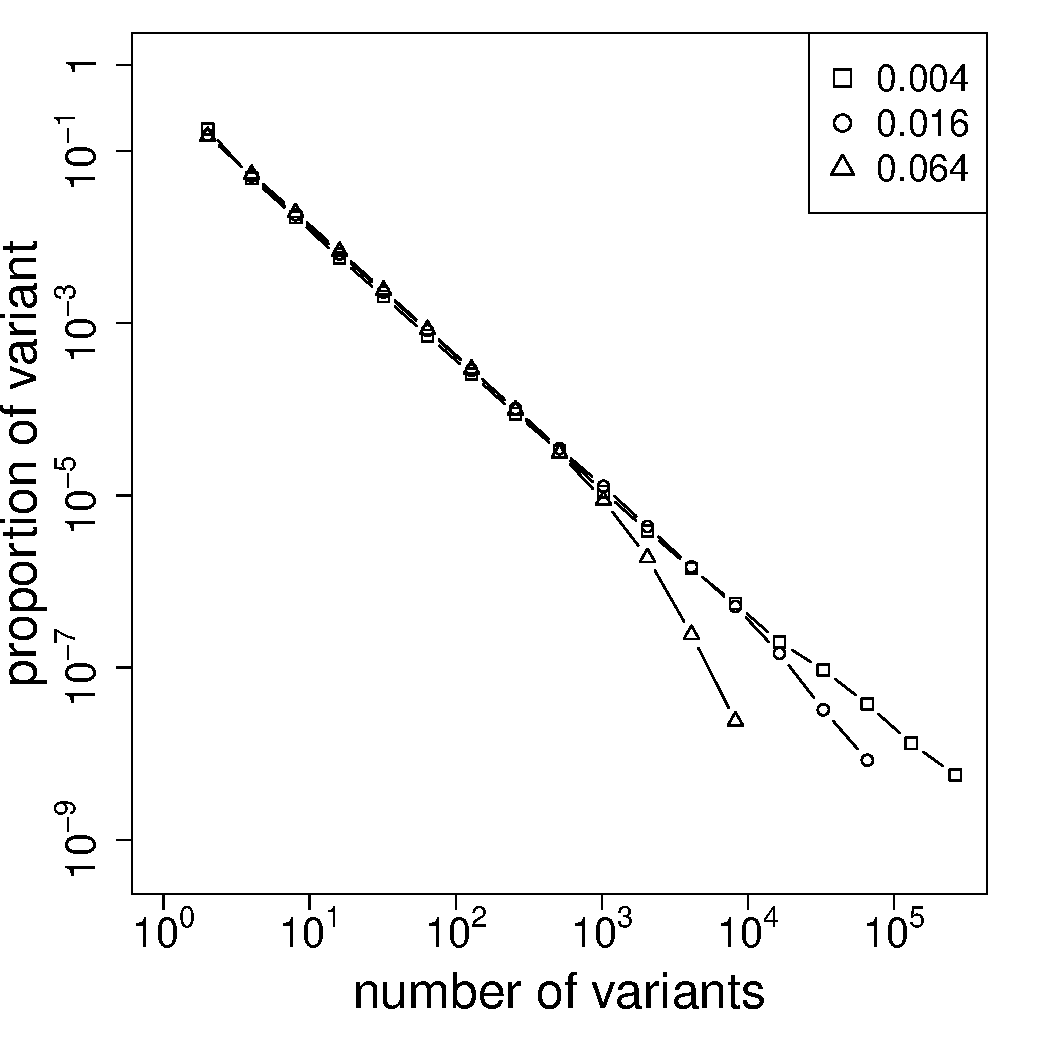
\includegraphics[width=7cm]{img/allmuRandMaxN250.pdf}&
		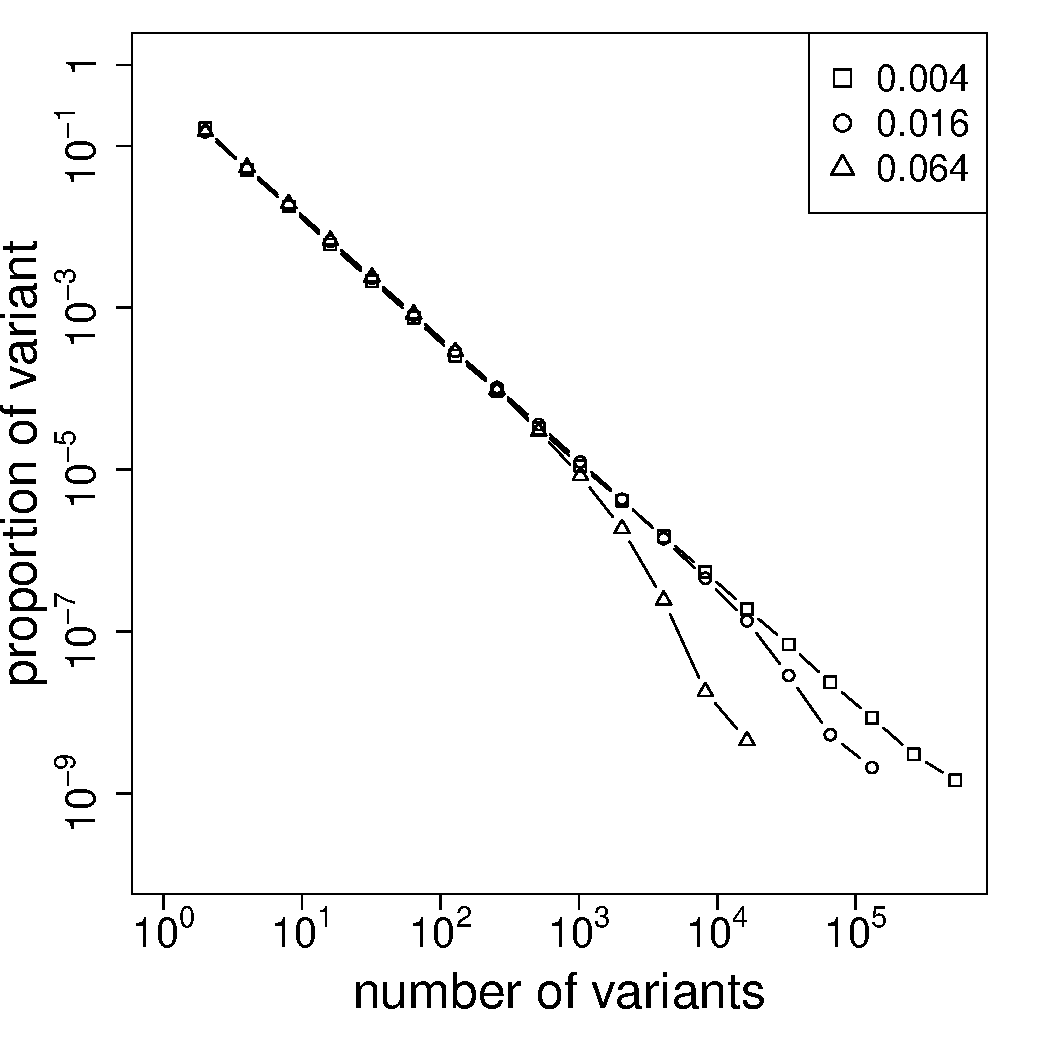
\includegraphics[width=7cm]{img/allmuRandMaxN500.pdf}
	\end{tabular}
	\caption{Distribution of proportions depending on the $\mu$ parameter with 250 agents (left) and 500 agents (right). Each plot is the mean obtenaid for 100 runs.\label{fig:allMutation}}
\end{figure}

We observe that the lower the mutation rate, the closer to a line the result is. This line corresponds to the ``power law" distribution explained in subsection~\ref{sec:tc:culturalTrans}, and is typical of the result obtained under the ``neutral hypothesis". In order to verify if the distribution is in fact a power-law, we follow the method proposed by~\cite{clauset2009powerlawdistributionsinempiricaldat} and the R implementation proposed by~\cite{gillespie_fitting_2015}. Briefly, two values are returned: a) the estimation of the $\alpha$ parameter of the power law equation $P(v)=C/v^\alpha $; b) a $p$-value testing the null-hypothesis that our data could have been generated from a power law distribution.

The table~\ref{tab:mualpha} summarizes the results obtained on all setups. Each value shown in the table is the mean values of 100 simulations. We see that in almost every case the null hypothesis cannot be rejected, which means that indeed the repartition of the price follows a power law. The only exception is for $\mu$ equal to $0.064$, where the $p$-value is less than $0.05$. In this last case the null hypothesis is rejected, and we therefore assume that the distribution does not follow a power law.

\begin{table}[!h]
	\caption{Mean $\alpha$ \& $sd$ are calculated on 100 runs for our results, and 5 runs for Bentley et. al. 2004. $pr$ is the percentage of run for which the $p$-value is less than 0.05, i.e. the percentage of runs for which we rejected the null-hypotheses stating that the distribution follow a power law.}
	\centering
	\begin{tabular}{cc|ccc}
		\multicolumn{2}{r}{}&\multicolumn{2}{c}{Our result}&\multicolumn{1}{c}{Bentley et. al. 2004}\\
			N&$\mu$ & $\alpha$ ($sd$) & $p$-value ($sd$ - $pr$) &$\alpha$ ($sd$)\\\hline
		250	&0.004&1.53 (0.03)&0.58 (0.24 - .01)&1.54 (0.02)\\
			&0.016&1.57 (0.02)&0.35 (0.28 - .05)&1.57 (0.01)\\
			&0.064&1.66 (0.01)&0.0 (0.00 - 1)&1.67 (0.01)\\\hline
		500	&0.004&1.50 (0.02)&0.59 (0.28 - .02 )&1.53 (0.03)\\
			&0.016&1.55 (0.03)&0.15 (0.17 - .10 )&1.61 (0.04)\\
			&0.064&1.78 (0.08)&0.0 (0.00 - 1)&1.81 (0.10)\\
	\end{tabular}
	\label{tab:mualpha}
\end{table}

For comparison purposes the results obtained by~\cite{bentley_random_2004} (which tested the ``neutral hypothesis'' with the same methodology) are added in the last column of table~\ref{tab:mualpha}. 

It allows us to statistically test our model and to compare it to other already existing in the literature. We show here that our model is consistent with the existing literature and thus with already observed and known social phenomenon.

%This suggest that we could successfully use this model to test data coming from Archaeological and Historical record and compare the to the same study to see if those data can come from similar processes.

%It appears that these results are highly similar to ours. We note also that our results match the ones presented in~\cite{mesoudi_random_2009} where only one value of $\mu$ was tested ($\mu = 0.008$). However, it is difficult to know if the slight differences observed between our work and those previous studies are statistically significant as the two previous studies rely on only five runs for the computation of the mean of $\alpha$ (against 100 in our case).
%
%Nonetheless, for high values of $\mu$, previous works report that the distribution of variant follow a power law~\cite{bentley_random_2004}. This claim is based on the fact that the estimated $\alpha$ (estimation based on linear regression on the log-log curve) has a high correlation coefficient. Recent works have shown that the use of correlation coefficient should be avoided~\cite{clauset2009powerlawdistributionsinempiricaldat}. Following these recent findings, our results preclude us to assume that the distribution of variant when $\mu$ is up to $0.064$ follow a power law . 
%
%An additional series of experiments is done to analyse how the system reacts when multiple goods are present. The mean values of $\alpha$ and $p$-value have been analysed for 3 innovation rates (0.004, 0.016, 0.064), 4 number of goods (1, 3, 6, 9), and 250 agents. However, due to the simplicity of the results and the space restriction we only report the analysis of the results here. 
%
%Visual analysis reveals that independently of the number of goods, the distributions obtained are exactly the same. Therefore it is no surprise that, for each innovation rate, the properties of the distribution of prices does not depend on the number of goods.


\subsubsection{Distribution of variants}

In order to understand the effect of introducing trading mechanisms, we compare first the distribution of values obtained in the ``trading model'' against the values obtained in the ``neutral model''. The figure~\ref{fig:2setDi}.a) presents the results obtained from 100 runs for each model. All runs rely on the same experimental setup using 3 goods, 500 agents and $\mu$ equal to 0.004. In all following graph  a variant is one price of one given good. The distributions are first computed for each good independently and then averaged together.

\begin{figure}[!h]
	\begin{center}
		\begin{tabular}{ccc}
		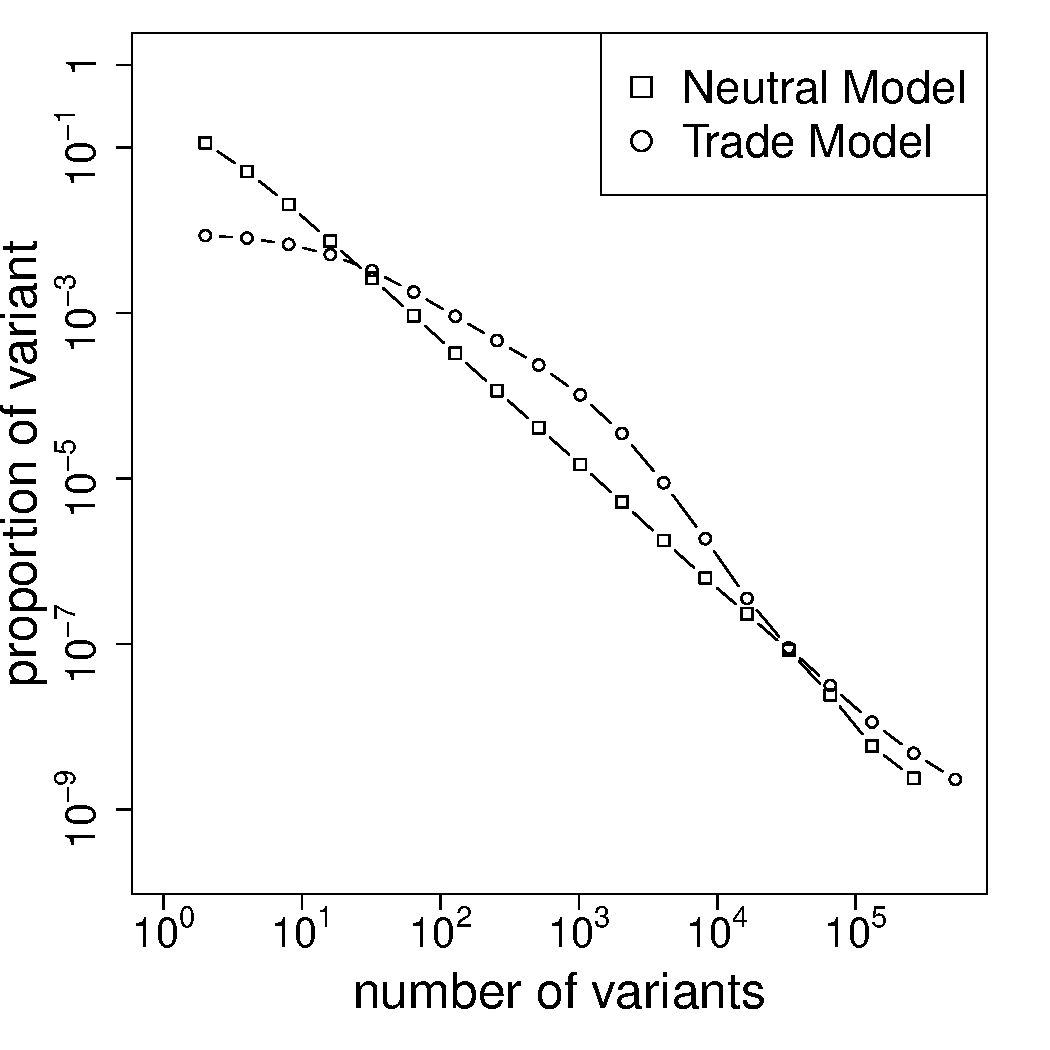
\includegraphics[width=5.2cm]{img/2SetupDistribA.pdf} &
		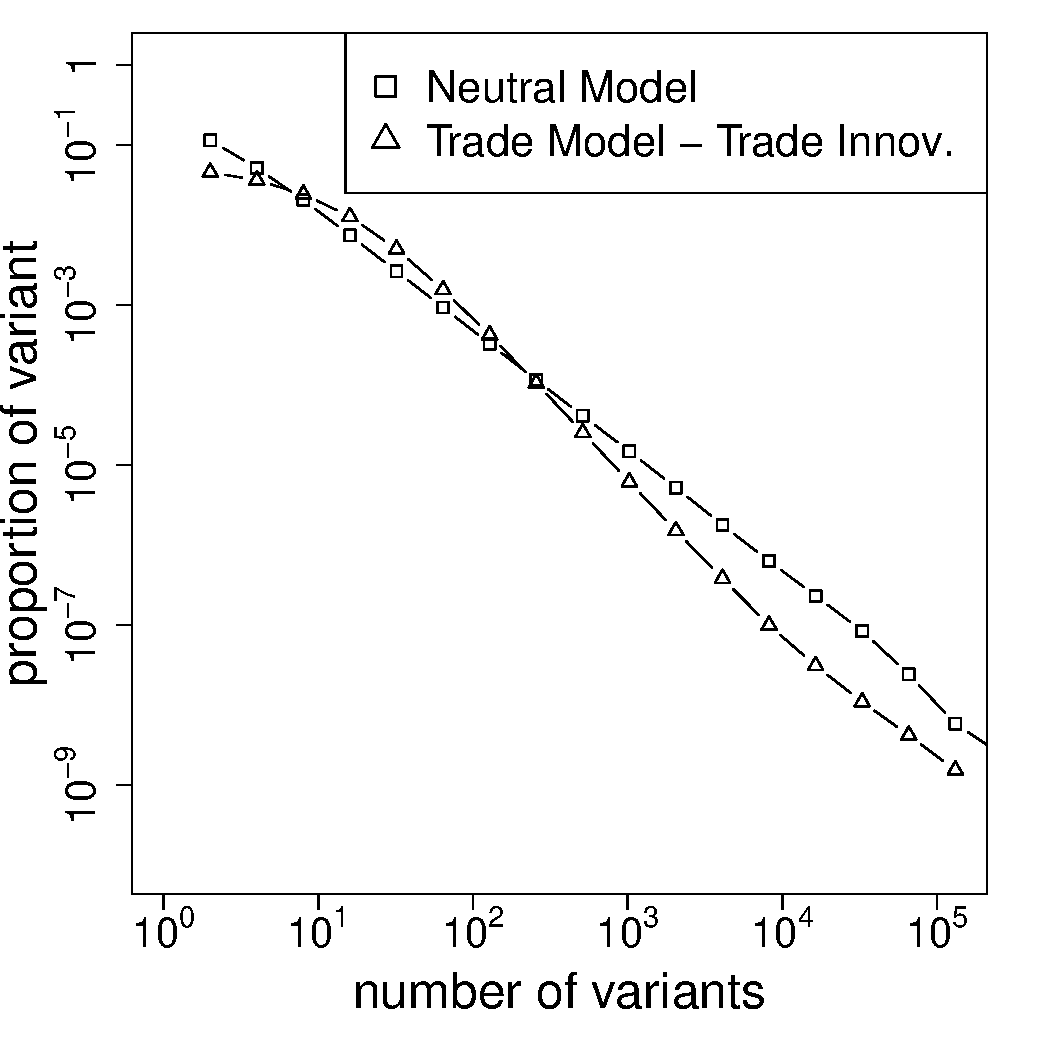
\includegraphics[width=5.2cm]{img/2SetupDistribB.pdf} &
		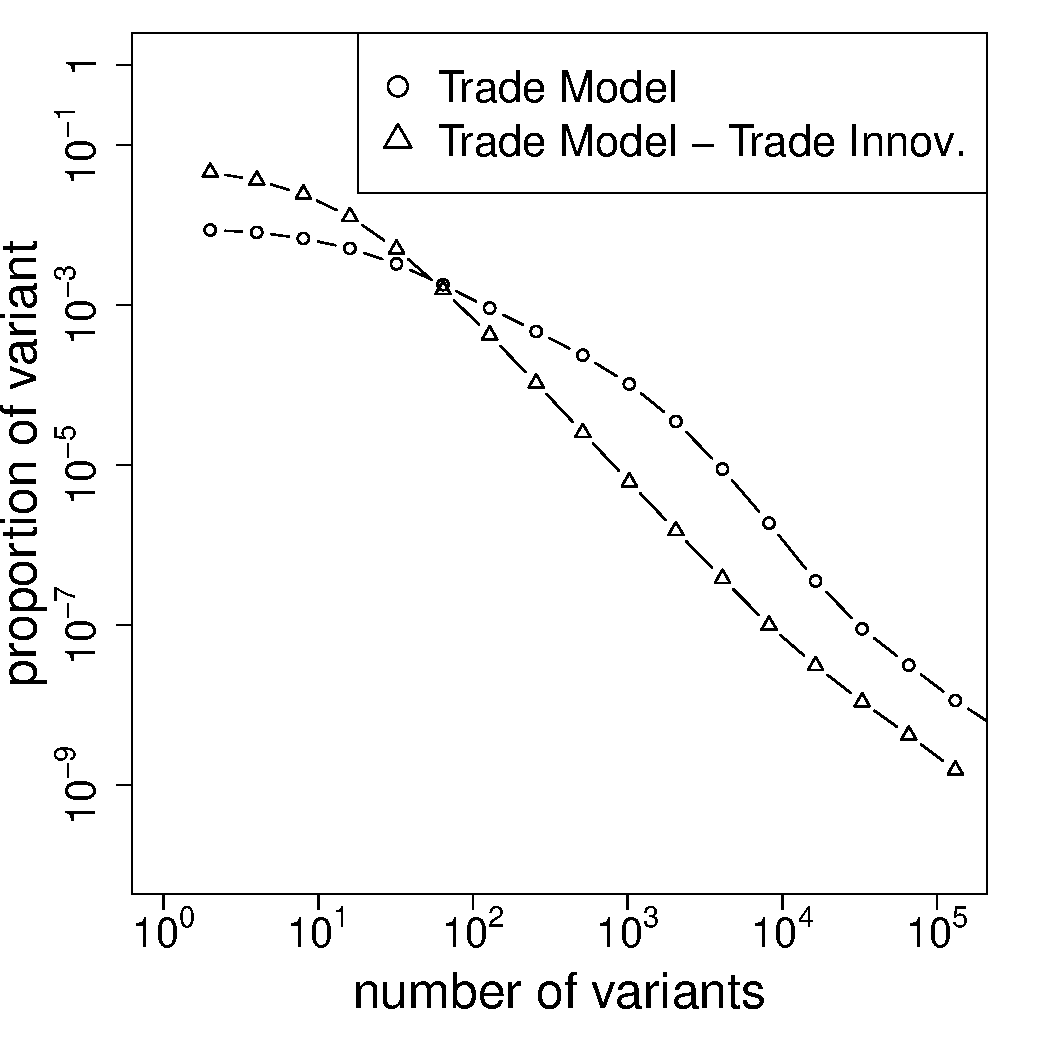
\includegraphics[width=5.2cm]{img/2SetupDistribD.pdf} \\
		a) & b) & c)  \\
		\end{tabular}

	\end{center}
	\caption{Frequencies distribution, where each points represent the mean for 100 runs, for: a) the neutral and the trading models.  b) the neutral model and the trading model without the trading innovation process. c) the trade model and the trade model without the trading innovation process.}
	\label{fig:2setDi}
\end{figure}

On figure~\ref{fig:2setDi}.a) it appears that the implementation of trade mechanisms leads to a distribution of prices departing from the neutral hypothesis. In more details, the frequencies distribution has a plateau of common prices (a number of prices share similar and high proportions), which shows that, when trade is taken into account, the most common variants are more diverse. 

In order to investigate which mechanism influences this departure from the neutral model, additional investigations have been performed. Here is presented the results of the analysis on the effect of the \emph{innovation} process of the trade model. To conduct this analysis the \emph{innovation} process of the trade model has been replaced by the \emph{innovation} process of the neutral model. 100 runs have been performed with this model on the same experimental setup. The results obtained are compared to the neutral model in figure~\ref{fig:2setDi}.b) and to the trade model in figure~\ref{fig:2setDi}.c). 

On figure~\ref{fig:2setDi}.b) it appears that the replacement of the innovation process leads to the creation of a distribution close to the one obtained with the neural model. On figure~\ref{fig:2setDi}.c) we observe a strong reduction in the size of the plateau and an important difference between the two distributions. This analysis highlights the importance of the \emph{innovation} process of the trading model in the distribution of prices. This mechanism, by preventing the creation of totally random new price, promotes the creation of few similar prices.

Moreover, it shows how the implementation of one particular trade mechanism can be tested and compared to an already well know model that is already used to understand available data. This suggests we could easily implement others trade mechanism, inspired or documented by archaeological data or historical sources, and compare their expected impact on the cultural distribution with regard to traditional cultural mechanism or other trade mechanism as those presented here. 


\subsubsection{Study of scores}

The results obtained with the trade model are studied in more detail by investigating the ability of the population to find the price most suited for exchanges. This is done by first measuring the score of all agents in each of the two different models. The figure~\ref{fig:scoreEvol} uses again the results obtained from 100 runs for each model where all runs rely on the same experimental setup using 3 goods, 500 agents and $\mu$ equal to 0.004. The figure is showing, as boxplots, the score computed thanks to equation (\ref{eq:score}) for all agents of all runs. The y-axis shows the score computed and the x-axis shows the timesteps. The left plot shows the results obtained in the ``neutral model'' and the right plot shows the results obtained in the ``trading model''.


\begin{figure}[!h]
	\centering
	\begin{tabular}{ c c}
		 Neutral Model & Trading Model \\
		 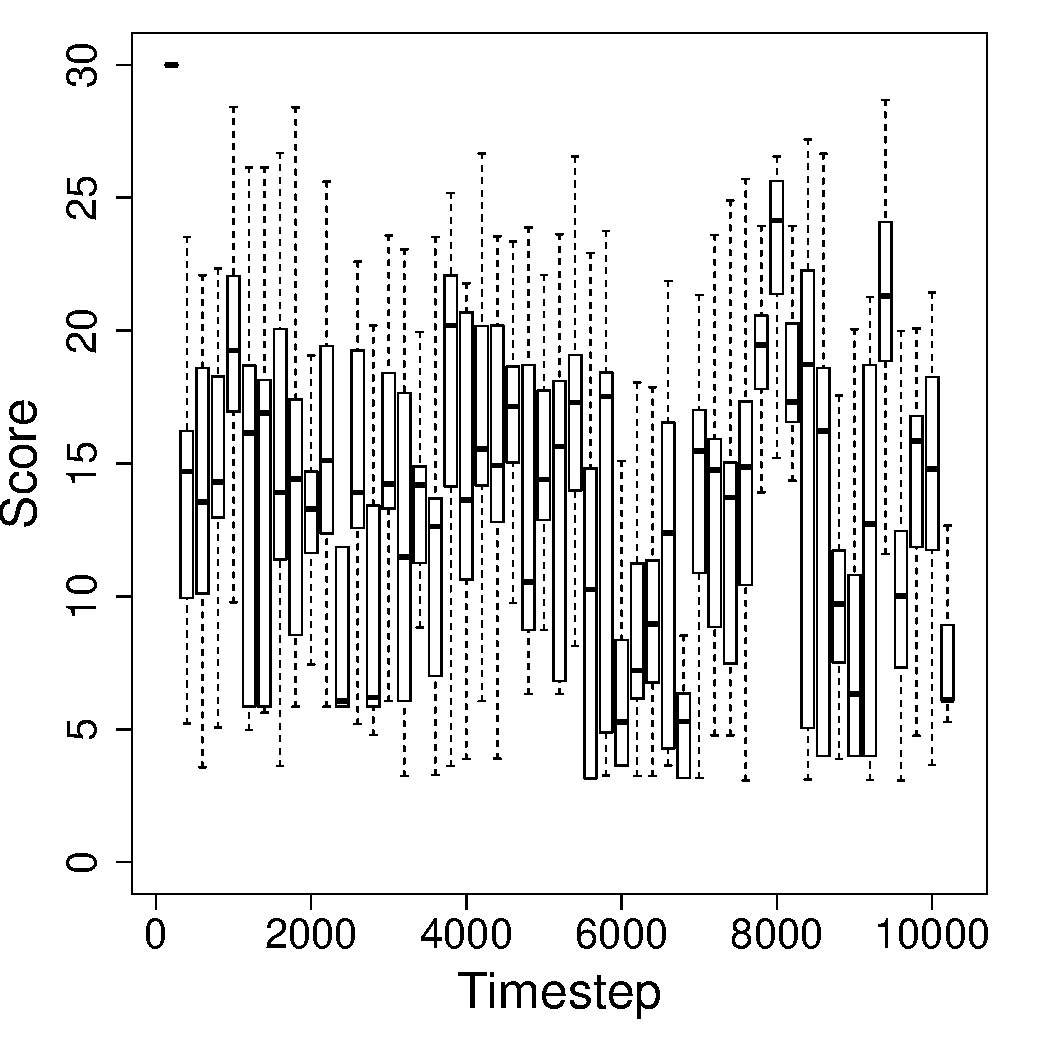
\includegraphics[width=5cm]{img/ScoreEvolutionForRandom-G3N500.pdf}
		 & 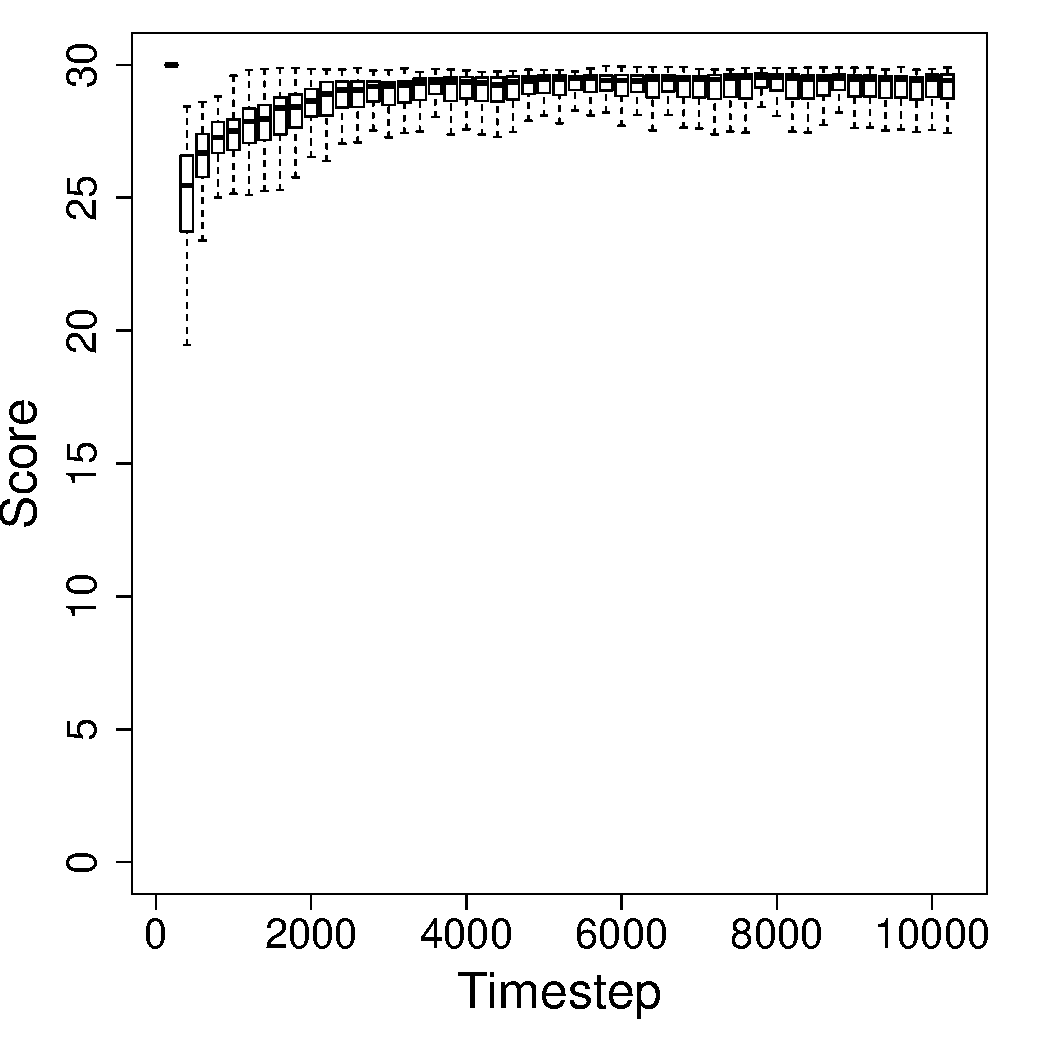
\includegraphics[width=5cm]{img/ScoreEvolutionForTrade-G3N500.pdf}

	\end{tabular}
	\caption{Evolution of the score within the two different models for two typical run with 500 agents and 3 goods evolving during 10000 timestep.}%%
	\label{fig:scoreEvol}
\end{figure}

As expected, the scores within the neutral model vary randomly. ``Trends'' may appear, where a bigger proportion of individuals adopt a better price that allow agents to reach better score (such as around iteration 8000), but such good score fall back as soon as another trend appears. However, with the trading model, the score of all the agents increase. As the selection mechanism allow them to know who has found better vectors of prices, they will progressively adopt prices vector that allow all of them to reach better scores. 

The previous figure showed the capacity for the trading model to increase its score but did not analyse the exact prices used. As explained in the subsection~\ref{sec:tc:trade} we expect that the trade \emph{cultural transmission} and \emph{innovation} processes will produce a convergence toward a set of price for each good that will allow agents to exchange optimally the good they produce with the other goods. To verify this assumption we analyse the prices reached during the simulations. These are presented in figure~\ref{fig:ratioEvol} for the 100 runs relying the experimental setup using 3 goods, 500 agents and $\mu$ equal to 0.004. For all runs, all agents and at each iteration we compute the difference between the price used by the agent $V_g$ and the optimal price $\tilde{V}_g$ (given by equation~\ref{eq:optimum}). The measures performed are presented as boxplots condensing the results for 100 runs.

\begin{figure}[!h]
	\begin{center}
		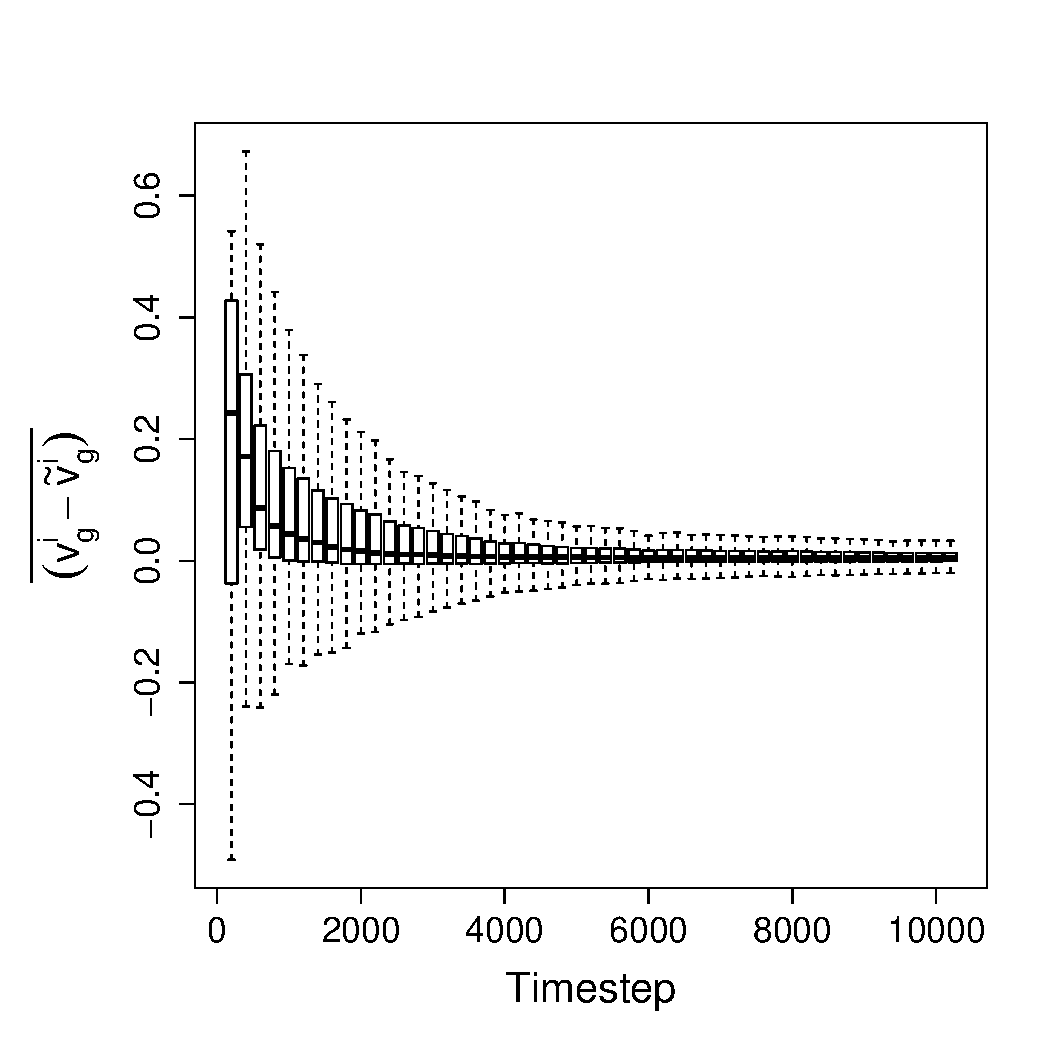
\includegraphics[width=7cm]{img/ClearingPriceDistanceEvolutionForTrade-G3N500.pdf}
	\end{center}
	\caption{Evolution of the mean of the difference between the estimated value $v^i_g$ and the optimal value $\tilde{v}^i_g$ (calculated with equation~\ref{eq:optimum}) for a good $g$ and an agent $i$. As the optimal value $\tilde{v}^i_g$ depends on which good is produced by $i$, the mean of the difference between the estimated price and the optimal one is computed between all the agents that produce the same good. The figure represents this mean computed at each timestep for each goods, for each groups of agents and for 100 runs in a setup with 500 agents and 3 goods. }
	\label{fig:ratioEvol}
\end{figure}

We observe that prices are indeed converging to the optimal prices which means that the agents within the trading model are indeed improving their scores by reaching the optimal prices. Notably, a similar variation of prices was observed in the closely related economical model of~\cite{gintis_emergence_2006}. This variation of the prices to the optimum offers an additional conformation of the validity of the trading model. 

\subsection{Summary}

With this model we propose a framework to simultaneously study cultural change and trade dynamics. The development of this framework was first aimed at simplicity which is achieved by the use of two vectors (quantity and value) and five processes (production, consumption, trade, cultural transmission and innovation). 
The second aim of the work conducted was to obtain a flexible framework which is possible since each of the processes can be implemented accordingly to the question studied. Both objectives were selected to provide a way to implement assumptions, hypotheses and hints made on the cultural and trading environment in the Roman Empire, where the culture dimension was tightly linked to the economics activity. We shown here how simple assumptions made at different level (see our implementation of the production, consumption, trade, cultural transmission and innovation mechanisms described in the Section~\ref{sec:tc:culturalTrans}~and~\ref{sec:tc:trade}) can be tested and compared. Those simple assumption could then easily be change by other made in the literature \cite{verboven2015structureandperformanceintheromaneconomymodelsmethodsandcasestudies}.

Moreover, we have shown the theoretical validity of this approach by reproducing expected results on both the cultural and trade side. On the cultural transmission side we have shown that the implementation of a ``neutral model" leads to the expected observations on the variants of the vector value: a power law. When implementing trading mechanisms we observe the convergence of prices to the expected values and the improvement of the scores of the agents.

%The successful implementation of a trading model within our framework shows that trading models can be viewed as a particular implementation of the cultural evolutionary framework. This aspect which has not been studied before, opens a new line of thinking on the weight of trade mechanisms within cultural change. Notably, we have shown that the implementation of trade mechanisms leads to a distribution of prices departing from the neutral hypothesis, which is the reference in the study of cultural changes. Within the trading model, the frequency distribution has a plateau of common prices (a number of prices share similar and high proportion), which shows that, when trade is taken into account, the most common variants are more diverse. Interestingly, we have not find references pointing at the ability of trade mechanisms to keep a relatively large diversity in the frequency distribution. We suspect that this is mainly because it is not common to compare results of trading models to other cultural evolution models. It would therefore be interesting to compare the frequency distributions obtained by our model and the ones observed in current or past economies. On the side of cultural transmission, the results obtained can also be compared to the ones obtained when prestige biased cultural transmission is used. The idea behind this last comparison, is that trade could be interpreted as a particular prestige biased cultural transmission and therefore be fully integrated within the cultural evolutionary frameworks.
%
%In future works more realistic scenarios can be studied in the same framework. Multiple implementations of the production mechanism can be studied so as to increase the number of goods per agent and include factors such as the meteorology or the various type of goods. Moreover, the introduction of the distinction between ``vital'' and ``common'' goods will be useful for the creation of models studying in further details the interaction between trade and cultural transmission. 
%
%Additionally, more complex dynamics can be looked for. The trading mechanism can be naturally implemented in different ways, each reflecting a specific theory, and thus allowing their comparisons. The cultural transmission mechanism also can be modified by including for example a crossover between the cultural trait of multiple agents. The trade network (which in this work can be interpreted as fully connected) can also be modified to study the effect of slow connections or the rupture of certain connections. The agent themselves could become more complex and be endowed with the ability to learn behaviours which would again produce more realistic simulations. Moreover, various populations can be envisioned, each with their distinctive characteristics regarding cultural transmission and trade. 

%Finally, in terms of analysis of the results, multiple factor could be taken into account. The rapidity of the fluctuation of prices is a good starting point for the establishment of economical studies. For the study of a population of agent in general, it can be interesting to analyse the number of agents active and the composition of the population.

\section{Conclusion}

In the this chapter we have argued that computer model and simulations are a good candidate to help historians and archaeologists in their quest for understanding the past. We have explain such point by taking the example of Biology and by showing that history is a perfect example of what kind of problem simulations can help us to solve and how. We have argued that computer simulations can help historian to select between different model already formalized by running numerical simulation, or they can help historian by given them a power tool to generate ``conceptual model'', or ``opaque thought experiment'' that allows to make hypothesis and assumptions explicit, to explore, compare and generate models of such hypothesis. 

We have then extensively illustrated such model with one that we have developed to study the co-evolution of trade and culture and by showing how we can test and already studied such model without relying on particular data. 

\section{Annex}

\subsection{Score \& Selection}

Formal computation of the score for agent $i$ and the good $j$:
\begin{equation}\label{eq:score}
s^i_j = \begin{cases}
 s_{max}=1 & \text{if $q^i_j = n_j$}\\
1 -\dfrac{\abs{q^i_j - n_j}}{ \sqrt{\abs{(q^i_j)^2-(n_j)^2}}} & \text{if $q^i_j \neq n_j$}
\end{cases}
\end{equation}



\begin{algorithm}
\caption{Selection Process}
\label{algo:selectionCulture}
	\begin{algorithmic}[1]
	\State	$ToGet = 0.2 \times \frac{\#Pop}{\#Good}$
	\For{$g \in Good$}
		\State	$ToReplace = \{\}$
                \While{$\#ToReplace < ToGet$} 
			\State $ j = SelectRand(Pop,g) $ \Comment{Select randomly an agent $j$ among the agents producing $g$}
			\State $X \sim U([0,1])$ \Comment{Draw a random number from the uniform distribution between 0 and 1}
			\If{$X>ComputeScore(j)$} \Comment{Select preferably the agents with the lowest scores}
				\State $ToReplace = \{ToReplace,j\}$
			\EndIf
		\EndWhile

                \While{$\#ToReplace > 0 $}
			\State $ j = SelectRand(ToReplace) $ 
			\State $ i = SelectRand(Pop,g) $  \Comment{Select randomly an agent $i$ among the agents producing $g$}
			\State $X \sim U([0,1])$ 
			\If{$ (X<ComputeScore(i))$} \Comment{Select preferably an agent $i$ with a high score}
				\If {$ (ComputeScore(i)>ComputeScore(j))$} \Comment{Verify that agent $i$ has a higher score than agent $j$}
					\State $CopyPrice(i,j)$
					\State $ToReplace = ToReplace - i$
				\EndIf
			\EndIf

		\EndWhile\
	\EndFor
\end{algorithmic}
\end{algorithm}


\subsection{Trade Mechanism}
The trading phase starts by the agent looking at a first random agent producing another good. 
Let $o$ be an agent producing $g$ who proposes a trade and $r$ an agent producing $k$ that receives the proposition. As explained earlier, each has a quantity of good $Q^o$ and $Q^r$. On the one side, $o$ wants to exchange a quantity $w_g^o$ of the good $g$ for a quantity $w_k^o$ of the good $k$. On the other side, $r$ wants to exchange a quantity $w_g^r$ of the good $g$ for a quantity $w_k^r$. The tuples $W^o$ and $W^r$ describe the quantities of goods wanted by agent $o$ and $r$ for one trade proposition and are defined by:  

\begin{equation}
	 W^o=(w_g^o = v_g^o,w_k^o= \frac{v_k^o}{v_g^o}), \quad
	 W^r=(w_k^r = v_k^r,w_g^r= \frac{v_g^r}{v_k^r}) 
	 \label{eq:trade}
\end{equation}

 Where $v_j^i$ are the estimated value of the good $j$ by the agent $i$ as defined earlier. 
The requested quantity of the non produced good is simply the ratio between the estimated value of the good requested and the estimated value of the produced good.


Once the quantities are defined, the agents declare that the trade is possible if :
\begin{align}
q_g^o >= w_g^o,\quad q_g^r <= w_g^o,\quad q_k^r >= w_k^o \label{eq:constraintQty}\\
w_g^o>=(q_g^r+w_g^r),\quad w_k^o<=w_k^r,\quad w_g^o<=w_g^r \label{eq:constraintWill}
\end{align}


The conditions \ref{eq:constraintQty} ensure that both agents have enough goods in their inventory to realise the trade while the conditions \ref{eq:constraintWill} ensure that the quantities of goods fit the will of both agents.

\begin{algorithm}
\caption{Trading Process for agent $o$}
\label{algo:trade}
	\begin{algorithmic}[1]
		\For{$j \in Goods \And j \neq produced^o $}
			\State $tradeAttempt = 0$
			\For{$r \in Pop \And produced^r = j \And tradeAttempt < TradeThreshold $}
				\If{$acceptableTrade(W_o,W_r)$}
					\State $trade(W_o,W_r)$
				\Else
					\State $tradeAttempt = tradeAttempt + 1$					
				\EndIf
			\EndFor
		\EndFor
\end{algorithmic}
\end{algorithm}



\bibliography{wsc,/home/scarrign/projects/PhD/doc/biblio/bib/phd}  
%\bibliographystyle{humannatOx}
\bibliographystyle{ieeetr}
\end{document}

